\documentclass[conference]{IEEEtran}



% *** GRAPHICS RELATED PACKAGES ***
%
\ifCLASSINFOpdf
  % \usepackage[pdftex]{graphicx}
  % declare the path(s) where your graphic files are
  % \graphicspath{{../pdf/}{../jpeg/}}
  % and their extensions so you won't have to specify these with
  % every instance of \includegraphics
  % \DeclareGraphicsExtensions{.pdf,.jpeg,.png}
\else
  % or other class option (dvipsone, dvipdf, if not using dvips). graphicx
  % will default to the driver specified in the system graphics.cfg if no
  % driver is specified.
  % \usepackage[dvips]{graphicx}
  % declare the path(s) where your graphic files are
  % \graphicspath{{../eps/}}
  % and their extensions so you won't have to specify these with
  % every instance of \includegraphics
  % \DeclareGraphicsExtensions{.eps}
\fi
% graphicx was written by David Carlisle and Sebastian Rahtz. It is
% required if you want graphics, photos, etc. graphicx.sty is already
% installed on most LaTeX systems. The latest version and documentation
% can be obtained at: 
% http://www.ctan.org/pkg/graphicx
% Another good source of documentation is "Using Imported Graphics in
% LaTeX2e" by Keith Reckdahl which can be found at:
% http://www.ctan.org/pkg/epslatex
%
% latex, and pdflatex in dvi mode, support graphics in encapsulated
% postscript (.eps) format. pdflatex in pdf mode supports graphics
% in .pdf, .jpeg, .png and .mps (metapost) formats. Users should ensure
% that all non-photo figures use a vector format (.eps, .pdf, .mps) and
% not a bitmapped formats (.jpeg, .png). The IEEE frowns on bitmapped formats
% which can result in "jaggedy"/blurry rendering of lines and letters as
% well as large increases in file sizes.
%
% You can find documentation about the pdfTeX application at:
% http://www.tug.org/applications/pdftex





\usepackage{amsmath}


\usepackage[utf8]{inputenc}
\usepackage{url}
\usepackage{hyperref}
\usepackage{graphicx}
% Packages for listings and color for code excerpts
\usepackage{listings}
\usepackage{color}
\definecolor{shadecolor}{rgb}{.9, .9, .9}

% stuff for nice looking JSON
\usepackage{xcolor}

\colorlet{punct}{red!60!black}
\definecolor{background}{HTML}{EEEEEE}
\definecolor{delim}{RGB}{20,105,176}
\colorlet{numb}{magenta!60!black}

\lstdefinelanguage{json}{
    basicstyle=\normalfont\ttfamily,
    numbers=left,
    numberstyle=\scriptsize,
    stepnumber=1,
    numbersep=8pt,
    showstringspaces=false,
    breaklines=true,
    frame=lines,
    backgroundcolor=\color{background},
    literate=
     *{0}{{{\color{numb}0}}}{1}
      {1}{{{\color{numb}1}}}{1}
      {2}{{{\color{numb}2}}}{1}
      {3}{{{\color{numb}3}}}{1}
      {4}{{{\color{numb}4}}}{1}
      {5}{{{\color{numb}5}}}{1}
      {6}{{{\color{numb}6}}}{1}
      {7}{{{\color{numb}7}}}{1}
      {8}{{{\color{numb}8}}}{1}
      {9}{{{\color{numb}9}}}{1}
      {:}{{{\color{punct}{:}}}}{1}
      {,}{{{\color{punct}{,}}}}{1}
      {\{}{{{\color{delim}{\{}}}}{1}
      {\}}{{{\color{delim}{\}}}}}{1}
      {[}{{{\color{delim}{[}}}}{1}
      {]}{{{\color{delim}{]}}}}{1},
}

\lstdefinestyle{mystyle}{
    %backgroundcolor=\color{shadecolor},
    %basicstyle=\ttfamily
    %basicstyle=\ttfamily\scriptsize
}


% acckorrect bad hyphenation here
\hyphenation{op-tical net-works semi-conduc-tor}


\begin{document}
\title{}


% author names and affiliations
% use a multiple column layout for up to three different
% affiliations
\author{}


% make the title area
\maketitle

% As a general rule, do not put math, special symbols or citations
% in the abstract
\begin{abstract}
\end{abstract}

\section{Introduction}


\section{Related work}


\section{Solution}

To solve these issues, we propose a modular architecture from which will stem a unified platform in which the benchmarks can be run. The main benefits of such a platform are twofold: to provide a common ground in which the middlewares can be benchmarked to ensure equal an playing field, and to ease the addition of other subsequent middlewares. This is achieved by factoring the common elements that go in the creation of any benchmarking application. The main building blocks of our architecture are visible in figure~\ref{fig:main_building_blocks}.

\begin{figure}[htbp!]
  \centering
  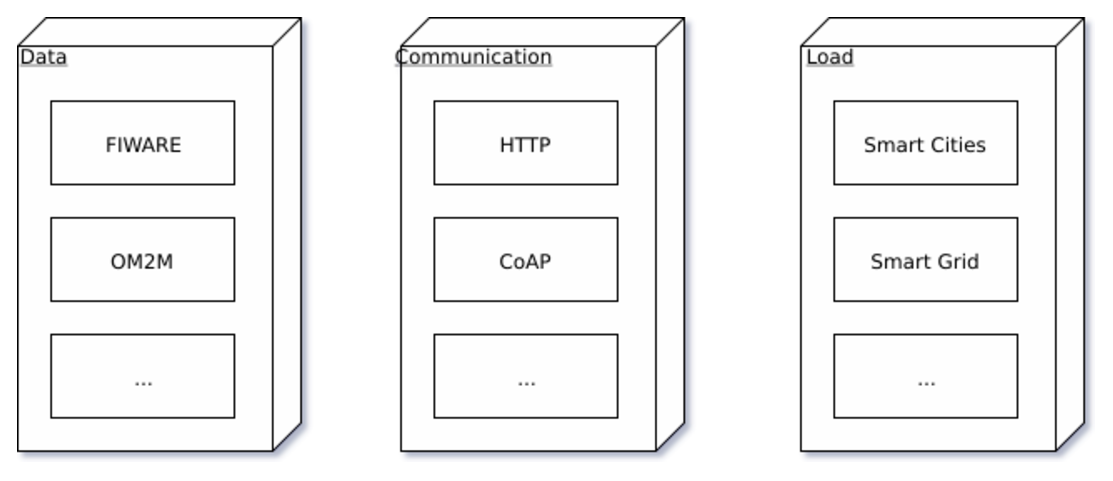
\includegraphics[width=\linewidth]{figures/benchmark_blocks.eps}
  \caption{Main architecture building blocks}
  \label{fig:main_building_blocks}
\end{figure}

The goal is to only implement what is necessary for a new entry in the benchmarking platform instead of using a similar implementation for each one. We propose a communication block where the communication protocols are lodged, such as HTTP or CoAP, and each has the methods implemented, such as POST or GET, so that they are totally platform independent and can be reused. If a new protocol is required to be added to the platform, its methods can be implemented without interfering with the remaining structure.

The data block is where the middleware specific functions reside, and each of these is responsible for implementing its data structure and bridging the gap to the protocols. Similarly to the data block, it is designed so that each is independent so that all can use the same communication methods implemented in the communication block. With a new entry, one can observe how the existing ones are structured, thereby speeding up the process and keeping it isolated without interfering with the existing setup. 

The load block will enable different types of IoT scenarios to be programmed and dynamically changed, so that we can attempt to mimic real world scenarios such as Smart Cities. Again, this should be independent from each of the other blocks so that the same workloads can be used throughout all middlewares and protocols, providing a basis for comparison and ensuring high flexibility.

Each building block will have several sub-blocks, which will correspond to a given class. In an initial phase, we attempted to create an application to benchmark the OM2M middleware with a basis on the work conducted in~\cite{pereira_benchmarking_2018} and \cite{cardoso_benchmarking_2017} , while keeping it as generic as possible to enable future middleware additions and follow our architecture guidelines. This resulted in the structure visible in~\ref{fig:class_diagram_om2m}.

\begin{figure}[htbp!]
  \centering
  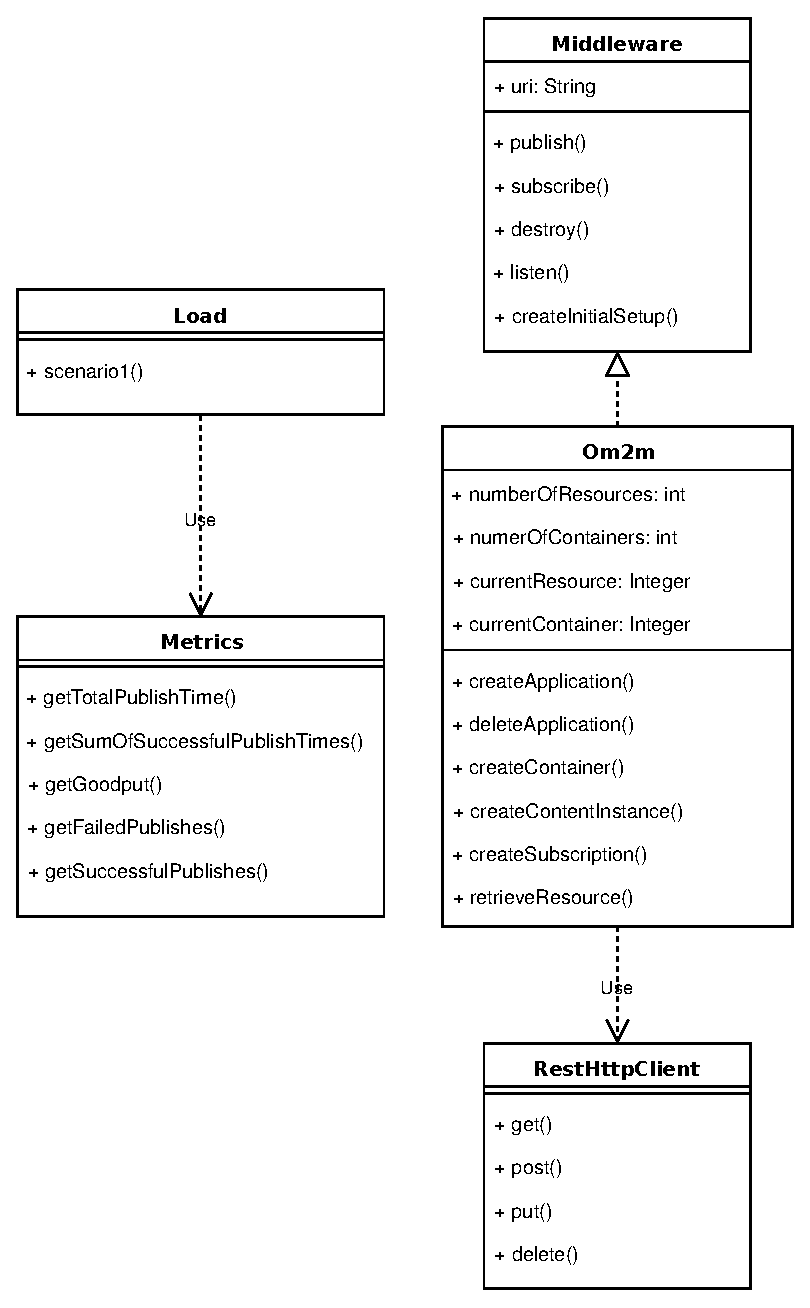
\includegraphics[width=\linewidth]{figures/class_diagram.eps}
  \caption{Class diagram for the initial platform stage}
  \label{fig:class_diagram_om2m}
\end{figure}

The main class is responsible for the load and most of the measurements. The load will consist of a certain number of publishes, with a certain message, at a given throughput. All can be easily defined by the user. It's implemented by way of a loop, with each cycle corresponding to a publish request, with sleeps in between to limit the throughput.

\begin{figure}[htbp!]
  \centering
  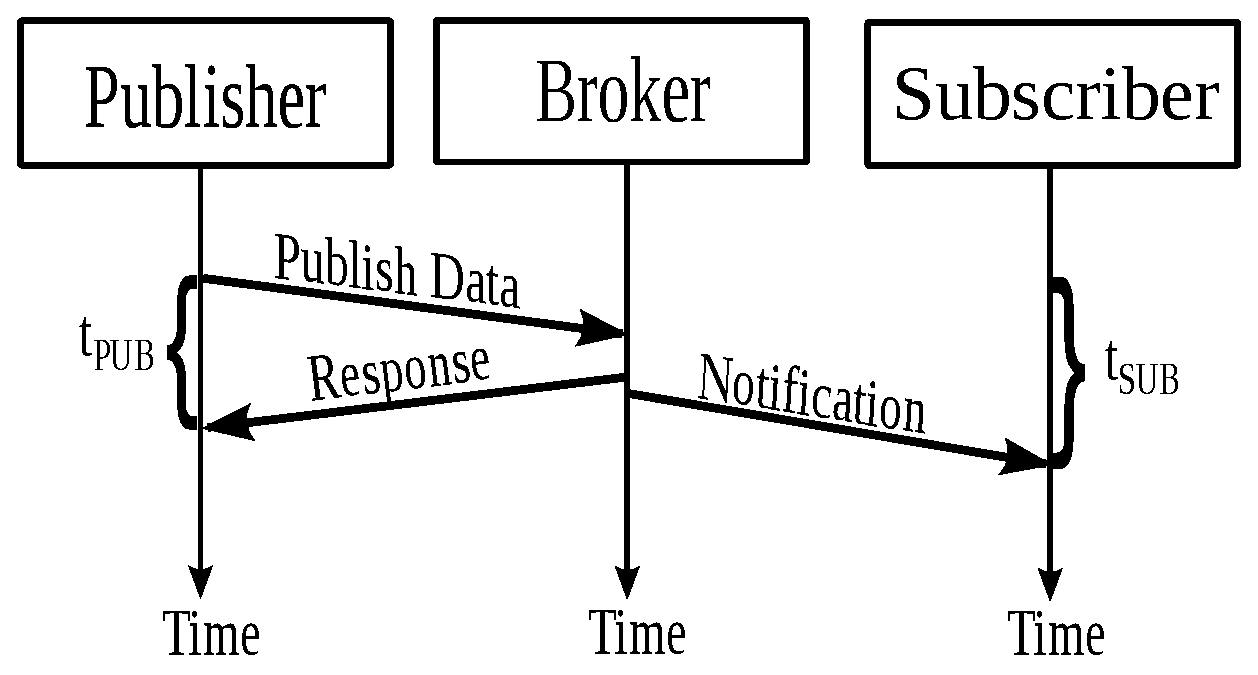
\includegraphics[width=\linewidth]{figures/pub_sub_time.eps}
  \caption{Publish and subscribe times~\cite{cardoso_benchmarking_2017}}
  \label{fig:pub_sub_time}
\end{figure}

The metrics currently implemented on are publish and subscribe time, both visible in~\ref{fig:pub_sub_time}, goodput, failed and successful publishes. Each publish time is simply the difference between sending the request and receiving the response from the broker, easily implemented in the main class by measuring the elapsed time of a single cycle in the load loop.
Goodput is measured by dividing the useful bytes of each message by each publish time. The useful bytes correspond to the full message that is assembled by each middleware. Let's take the Om2m class as an example. Here, a publish request corresponds to the creation of a content instance of the container where we wish to publish. Therefore, the \textbf{createContentInstance()} method will take the message as input and create the appropriate data structure, such as in~\ref{lst:application_creation} for creating an application, to be sent as payload for a certain protocol, e.g., HTTP\@.

\begin{lstlisting}[linewidth=\columnwidth, caption=JSON payload for application creation, captionpos=b, label=lst:application_creation, language=json]
{
   "m2m:ae": {
     "api": "app-sensor",
     "rr": "false",
     "lbl": ["Type/sensor", "Category/temperature", "Location/home"],
     "rn": "MY_SENSOR"
   }
}
\end{lstlisting}

This will be returned to the calling publish method, in order for it to know the payload size for that particular middleware publish request. Since this class extends the \textbf{middleware} superclass, this method is always present and always has the same return values, providing generic metrics.
Following this, we have the failed and successful publishes. In order to determine the whether a certain request was successful or not, some level of analysis must be conducted to the response provided by the broker. Naturally, this is protocol dependent, so in order to create a layer of abstraction, the basic communication methods of the used protocol, such as \textbf{POST} or \textbf{PUT} must return the broker response, in order for the Om2m class to be able to interpret if a publish was successful or not. This way, it will then return to the main class a generic indicator, independent of protocol, indicating its success or failure. 
Lastly, we have subscribe time which is implemented differently, as it potentially relies on times registered at different machines. In order for the subscriber to register the times, a listener must be created for the protocol it is expecting to receive. This listener will be in charge of registering the times at which the notification arrive, meaning this metric is implemented at the protocol level.

Moving on we have the \textbf{Middleware} superclass. Here the goal is to provide the methods that all middlewares are expected to implement and any attributes that are common as well. We therefore chose to have an \textbf{uri} to identify where it will be located on the network. The \textbf{publish()} and \textbf{subscribe()} methods are evident as we are dealing with publish/subscribe scenarios. The \textbf{destroy()} method provides a way to clear any created resources so that the experiment may be conducted again on a clean broker. Next, we have \textbf{listen()}, which is for the subscriber to call so that it may receive and parse notifications as needed, and register their arrival times. Finally, \textbf{createInitialSetup()} is for registering resources, such as applications in the case of OM2M, the number of which is defined by the user.

Then, we come to the protocol classes. Currently, only HTTP is implemented in the \textbf{RestHttpClient()}, but others may be added in the future, such as CoAP or MQTT\@. The four methods are ubiquitous across several applications, and typically most middelwares which rely on HTTP will make use of these. 


\section{Evaluation}


\section{Conclusion}



% trigger a \newpage just before the given reference
% number - used to balance the columns on the last page
% adjust value as needed - may need to be readjusted if
% the document is modified later
%\IEEEtriggeratref{8}
% The "triggered" command can be changed if desired:
%\IEEEtriggercmd{\enlargethispage{-5in}}

% references section

% can use a bibliography generated by BibTeX as a .bbl file
% BibTeX documentation can be easily obtained at:
% http://mirror.ctan.org/biblio/bibtex/contrib/doc/
% The IEEEtran BibTeX style support page is at:
% http://www.michaelshell.org/tex/ieeetran/bibtex/
%\bibliographystyle{IEEEtran}
% argument is your BibTeX string definitions and bibliography database(s)
%\bibliography{IEEEabrv,../bib/paper}
%
% <OR> manually copy in the resultant .bbl file
% set second argument of \begin to the number of references
% (used to reserve space for the reference number labels box)

\bibliographystyle{unsrt}
\bibliography{biblio}


% that's all folks
\end{document}


%%% Local Variables:
%%% mode: latex
%%% TeX-master: t
%%% End:

